\chapter{Despliegue en la nube con AWS}

\section{Amazon web services}

\begin{figure}[H]
    \centering
    
\includegraphics[width=40mm]{memoria/LaTeX/img/despliegue/aws2.png}
    \caption{AWS}
\end{figure}

\subsection{¿Qué es AWS?}
Amazon Web Services es una colección de servicios de computación en la nube que en conjunto forman una plataforma de computación en la nube, ofrecidas a través de Internet por Amazon.com.

\subsection{¿Por qué AWS?}
La cuestión de porque hemos elegido amazon web service como servicio de computación en la nube no es otra que por el gran impacto que esta teniendo en el mundo laboral, al margen de sus competidores directos como son Azure y Google Cloud.

Otro factor que juega a favor de AWS con respecto a sus competidores es que a la hora de desplegar una aplicación en la nube la experiencia de usuario me resulta mucho mas intuitiva que la de sus competidores. También debo destacar la importancia de tener un buen soporte como del que AWS dispone, donde en cualquier momento te resuelven las posibles dudas que tengas a la hora de desplegar la aplicación.

Por último y como factor de bastante importancia para aquellos pequeños emprendedores que quiera empezar a desarrollar sus ideas, es el bajo coste que supone tener una aplicación desplegada en la nube de amazon. Por el momento, el primer año de tu cuenta en AWS es gratuita, restringida a ciertas limitaciones.

\subsection{¿Quien lo utiliza?}

Cada vez son más las empresas que deciden utilizar la computación en la nube ya que desde 2006, , Amazon Web Services proporciona servicios de infraestructura de TI para empresas en forma de servicios web.

Uno de los principales beneficios de la computación en la nube es la oportunidad de reemplazar importantes gastos de infraestructura con costes reducidos que se escalan dependiendo de la dimensión de su negocio.

Gracias a la nube, las empresas ya no tienen que planificar ni adquirir servidores y otra infraestructura de TI con semanas o meses de antelación. Pueden disponer en cuestión de minutos de cientos o de miles de servidores y ofrecer resultados más rápidamente.

Hoy en día, Amazon Web Services proporciona una plataforma de infraestructura escalable, de confianza y de bajo costo en la nube que impulsa cientos de miles de negocios de 190 países de todo el mundo. Con centros de datos en Estados Unidos, Europa, Brasil, Singapur, Japón y Australia.

A continuación enumeraremos algunas de las empresas con más éxito en AWS:

\begin{enumerate}
     \item \textbf{Amazon.com: } Es el minorista online más grande del mundo. En 2011, Amazon.com pasó de utilizar el backup en cinta a usar Amazon S3 en la cloud para realizar copias de seguridad de la mayoría de las bases de datos de Oracle de las que se encarga. Mediante el uso de AWS, Amazon.com logró eliminar el software de backup y experimentó una mejora de desempeño 12 veces mayor, de forma que pudo reducir el tiempo de restablecimiento de 15 a 2,5 horas aproximadamente en situaciones seleccionadas.
    \item \textbf{Netflix: } El referente de la televisión en streaming, usa AWS para proporcionar miles de millones de horas de vídeo casa mes a sus mas de 60 millones de suscriptores. Así puede hacer uso de miles de servidores y terabites de almacenamiento en cuestión de minutos para que sus usuarios puedan ver series y películas desde cualquier parte del mundo en sus tabletas o teléfonos móviles.
    \item \textbf{Dropbox: } El famoso y conocido servicio de alojamiento de archivos multiplataforma en la nube, utiliza hasta el momento AWS como repositorio para almacenar todos los archivos que los usuarios de Dropbox suben a la red. 
    \item \textbf{Bankinter: } Utiliza AWS como de su aplicación de simulación de riesgo crediticio, pasando de 23 horas a 20 minutos.
    \item \textbf{FC Barcelona: }Su sitio web, que aloja más de 6 000 páginas y 12.000 fotos digitales, también usa AWS para su mantenimiento.
    \item \textbf{Harvard Medical School} Desarrolla nuevos modelos de pruebas de genomas en tiempo récord. 
    \item \textbf{Mapfre: }Ahorró 1,3 millones de euros en infraestructura y redujo el desarrollo de semanas a días
    
\end{enumerate}

\section{Lanzar una instancia en AWS}

Ahora que ya sabemos en detalle de lo que consiste AWS, antes de poder subir nuestra aplicación a producción debemos de crear una instancia en AWS.

Estos son los pasos a tener en cuenta a la hora de crear una instancia en AWS:

\begin{itemize}
    \item \textbf{Paso1. Crear Key Pairs} Los Key Pairs se utilizan para iniciar sesión de forma segura en los servicios de AWS. Crearemos un Key Pairs para acceder a nuestra instancia de EC2.
\begin{enumerate}
    \item Para crear nuevos pares de claves, navegue hasta AWS Console y luego haga clic en EC2.
    \begin{figure}[H]
    \centering
    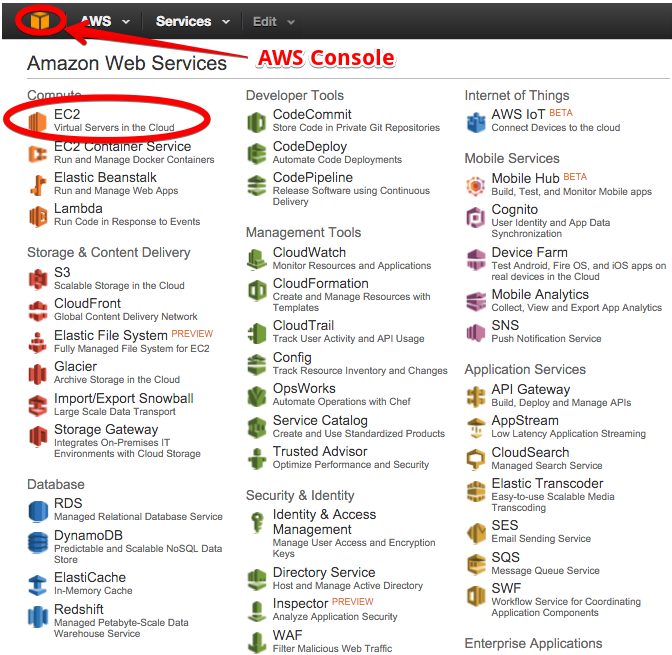
\includegraphics[width=60mm]{memoria/LaTeX/img/despliegue/paso1_1.png}
    \caption{Paso 1.1}
    \end{figure}
    \item En el panel izquierdo, haga clic en Key Pairs, luego haga clic en Crear Key Pairs
     \begin{figure}[H]
    \centering
    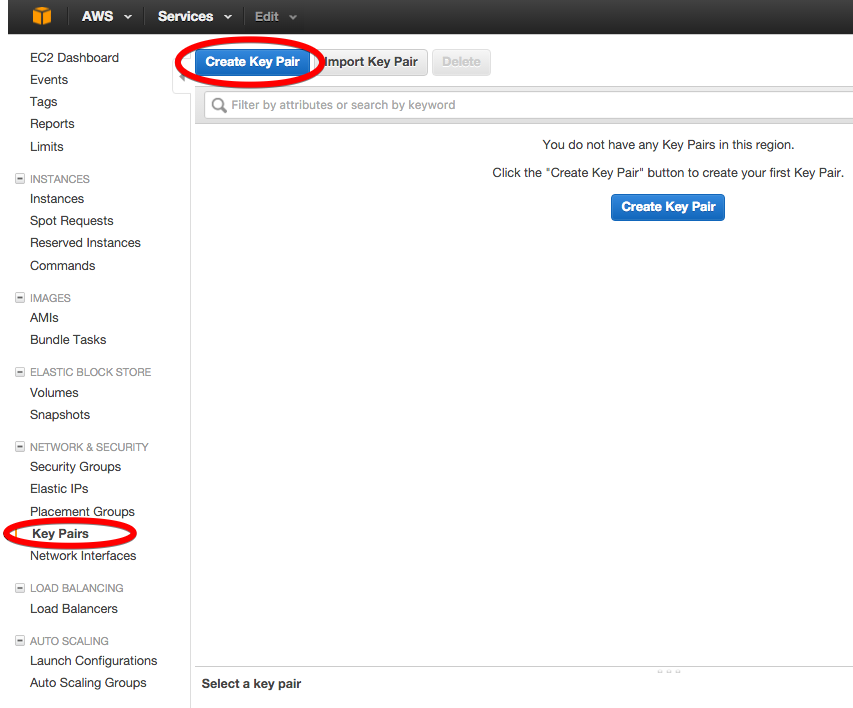
\includegraphics[width=60mm]{memoria/LaTeX/img/despliegue/paso1_2.png}
    \caption{Paso 1.2}
    \end{figure}
    \item Ingrese un nombre para su clave, luego haga clic en Crear Key Pairs. El Key Pairs se descargará automáticamente. Debe mover esta clave a un directorio diferente.
    
    Importante: Deberá cambiar los permisos de esta clave para que sean de solo lectura, consulte el siguiente código:
    \begin{lstlisting}
    chmod 400 youKeyName.pem
    \end{lstlisting}
\end{enumerate}
    \item \textbf{Paso 2. Lanza una instancia de EC2 con Bitnami} En este paso, lanzaremos una instancia de EC2 desde Amazon Machine Image (AMI). 
    
    Con AMI, puede activar una instancia de EC2 que esté lista para el desarrollo sin demasiada configuración. Bitnami proporciona una imagen MEAN preconfigurada, que usaremos para configurarlo rápidamente.
    
    \begin{enumerate}
    \item Primero, navegue a la consola de AWS, haga clic en AWS Marketplace.
    \begin{figure}[H]
    \centering
    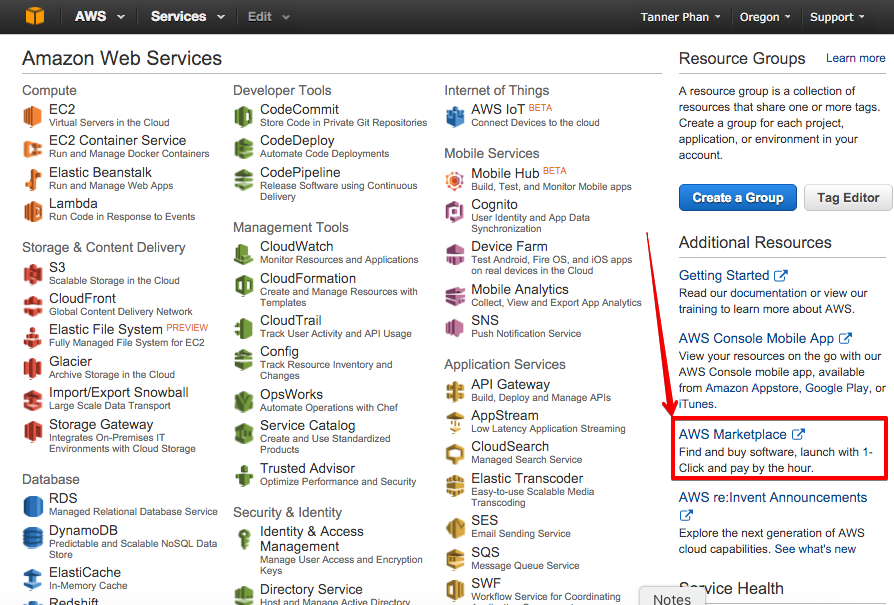
\includegraphics[width=60mm]{memoria/LaTeX/img/despliegue/paso2_1.png}
    \caption{Paso 2.1}
    \end{figure}
    \item Search for MEAN powered by Bitnami, then select the 64-bit AMI to continue.
    \begin{figure}[H]
    \centering
    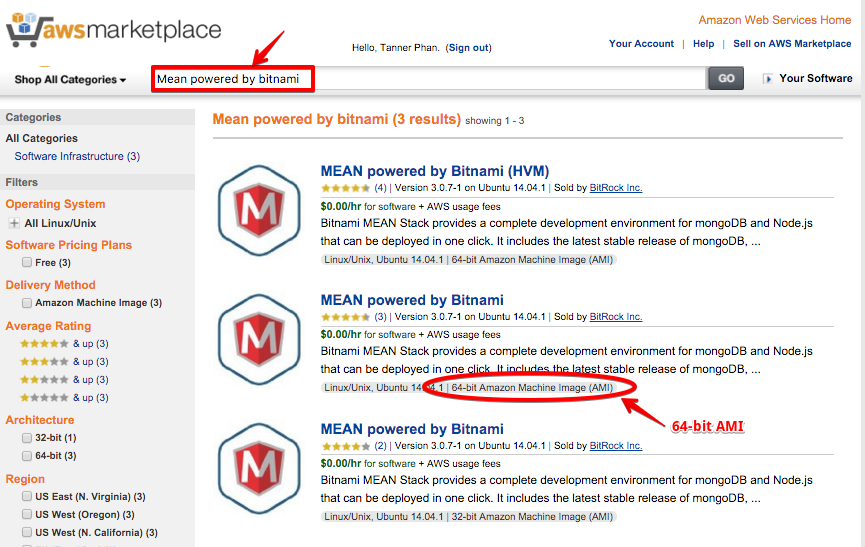
\includegraphics[width=60mm]{memoria/LaTeX/img/despliegue/paso2_2.png}
    \caption{Paso 2.2}
    \end{figure}
    \item En Pricing Details con el fin de obtener la mejor velocidad de entrega, seleccione la región más cercana y luego haga clic en Continuar.
    \begin{figure}[H]
    \centering
    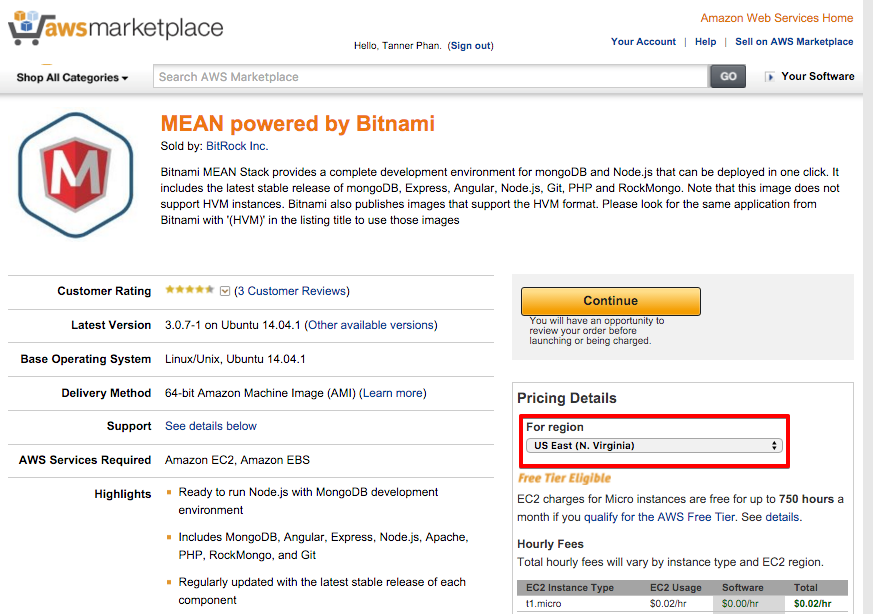
\includegraphics[width=60mm]{memoria/LaTeX/img/despliegue/paso2_3.png}
    \caption{Paso 2.3}
    \end{figure}
    \item Para el grupo de seguridad, elija Crear nuevo según la configuración del vendedor.
    \item Asegúrese de tener los siguientes métodos de conexión:
    \begin{lstlisting}
     1.SSH, My IP
     2.HTTP, Anywhere
     3.HTTPS, Anywhere
    \end{lstlisting}
    \begin{figure}[H]
    \centering
    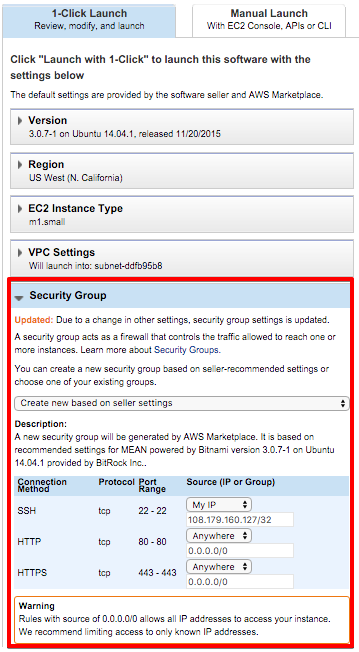
\includegraphics[width=60mm]{memoria/LaTeX/img/despliegue/paso2_5.png}
    \caption{Paso 2.5}
    \end{figure}
    \item Selecciones la Key Pair que creaste en el paso 1.
    \begin{figure}[H]
    \centering
    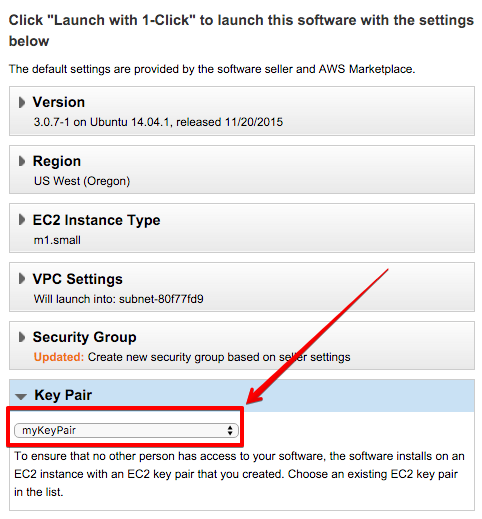
\includegraphics[width=60mm]{memoria/LaTeX/img/despliegue/paso2_6.png}
    \caption{Paso 2.6}
    \end{figure}
    \item Finalmente, haga clic en Iniciar, para iniciar la instancia.
    \end{enumerate}
    \item \textbf{Paso 3. Conéctate a tu EC2} Para conectarte por SSH a su instancia, necesitará la IP pública de su instancia y el Key Pair que creó.
    \begin{enumerate}
    \item Dentro de EC2, haga clic en Instancias, seleccione la instancia recién iniciada en el paso anterior y luego haga clic en Conectar.
    \item Copie el código que aparece marcado en rojo en la siguiente imagen.
    \begin{figure}[H]
    \centering
    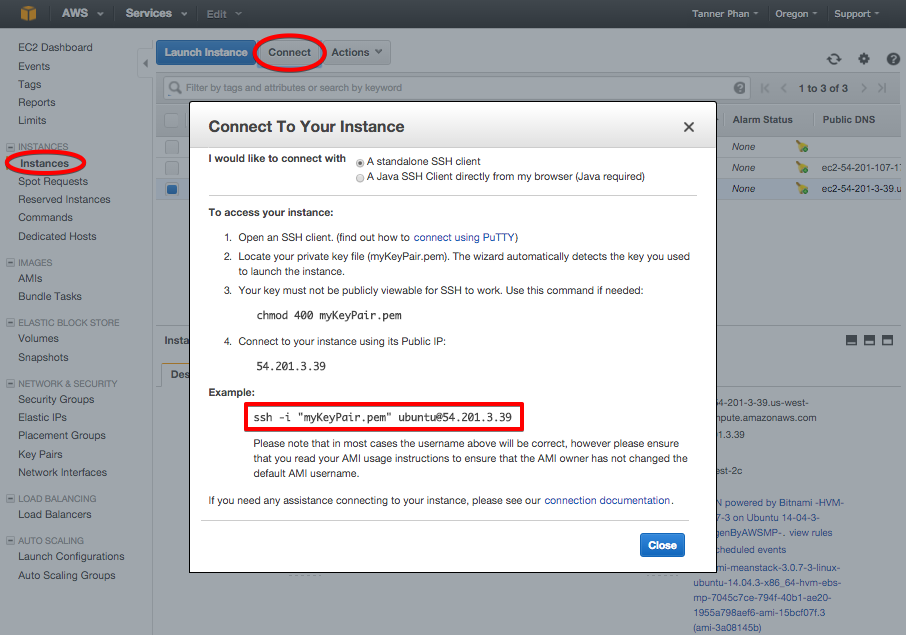
\includegraphics[width=60mm]{memoria/LaTeX/img/despliegue/paso3_2.png}
    \caption{Paso 3.2}
    \end{figure}
    \item En su terminal, navegue hasta el directorio donde está guardado su par de claves, luego pegue el último paso del código.
    \begin{figure}[H]
    \centering
    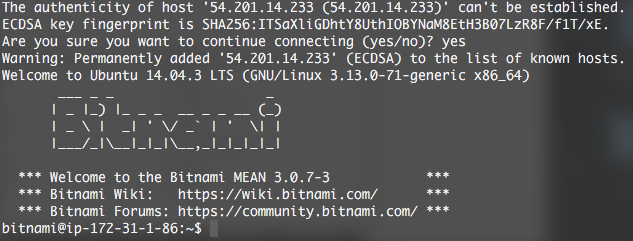
\includegraphics[width=60mm]{memoria/LaTeX/img/despliegue/paso3_3.png}
    \caption{Paso 3.3}
    \end{figure}
    \end{enumerate}
    
    \item \textbf{Paso 4. Conseguir un dominio gratuito} Una vez que ya tenemos la instancia creada y hemos sido capaces de conectarnos a ella por SSH, llega el momento de conseguir un dominio para que los usuarios se puedan conectar a la aplicación lo más fácil posible.
    El dominio que he utilizado es un dominio gratuito, proporcionado por el portal freedom.com, la forma de conseguirlo es la siguiente:
    
    \begin{enumerate}
        \item Vaya a https://my.freenom.com e inscríbase.
        \begin{figure}[H]
        \centering
        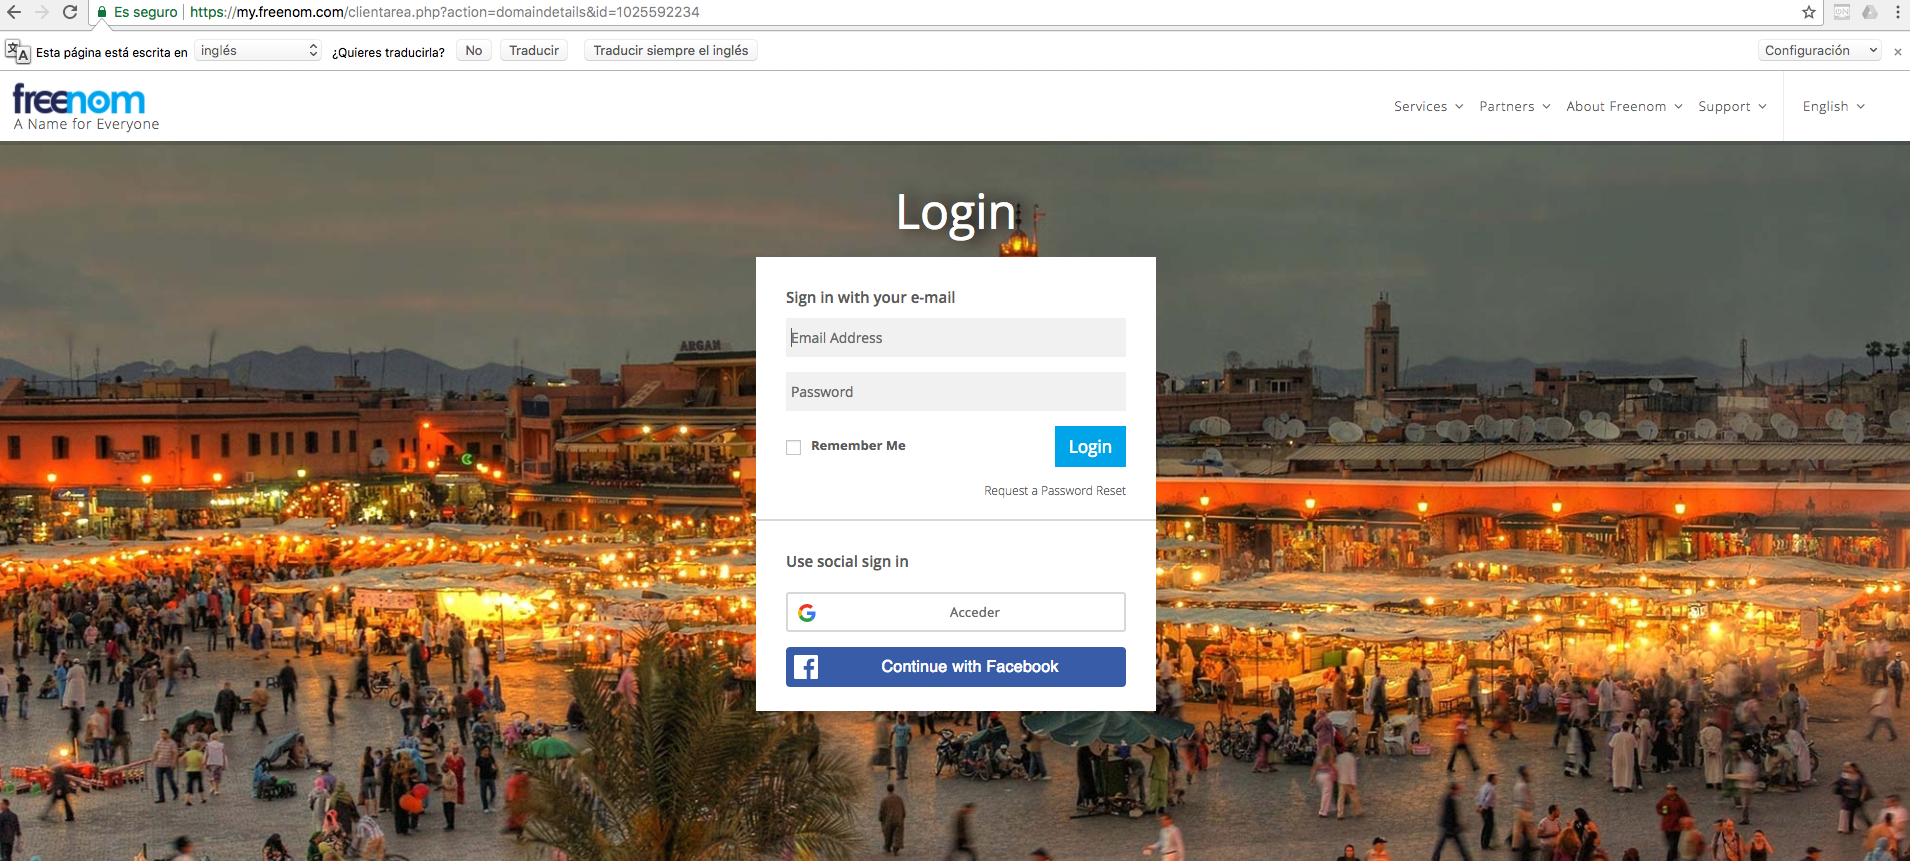
\includegraphics[width=80mm]{memoria/LaTeX/img/despliegue/dominiofree/pas1_1.png}
        \caption{Paso 1.1}
        \end{figure}
         \item Una vez que nos hemos logueado, tenemos que ir a la sección de My Domains y allí elegir un dominio que este disponible.
        \begin{figure}[H]
        \centering
        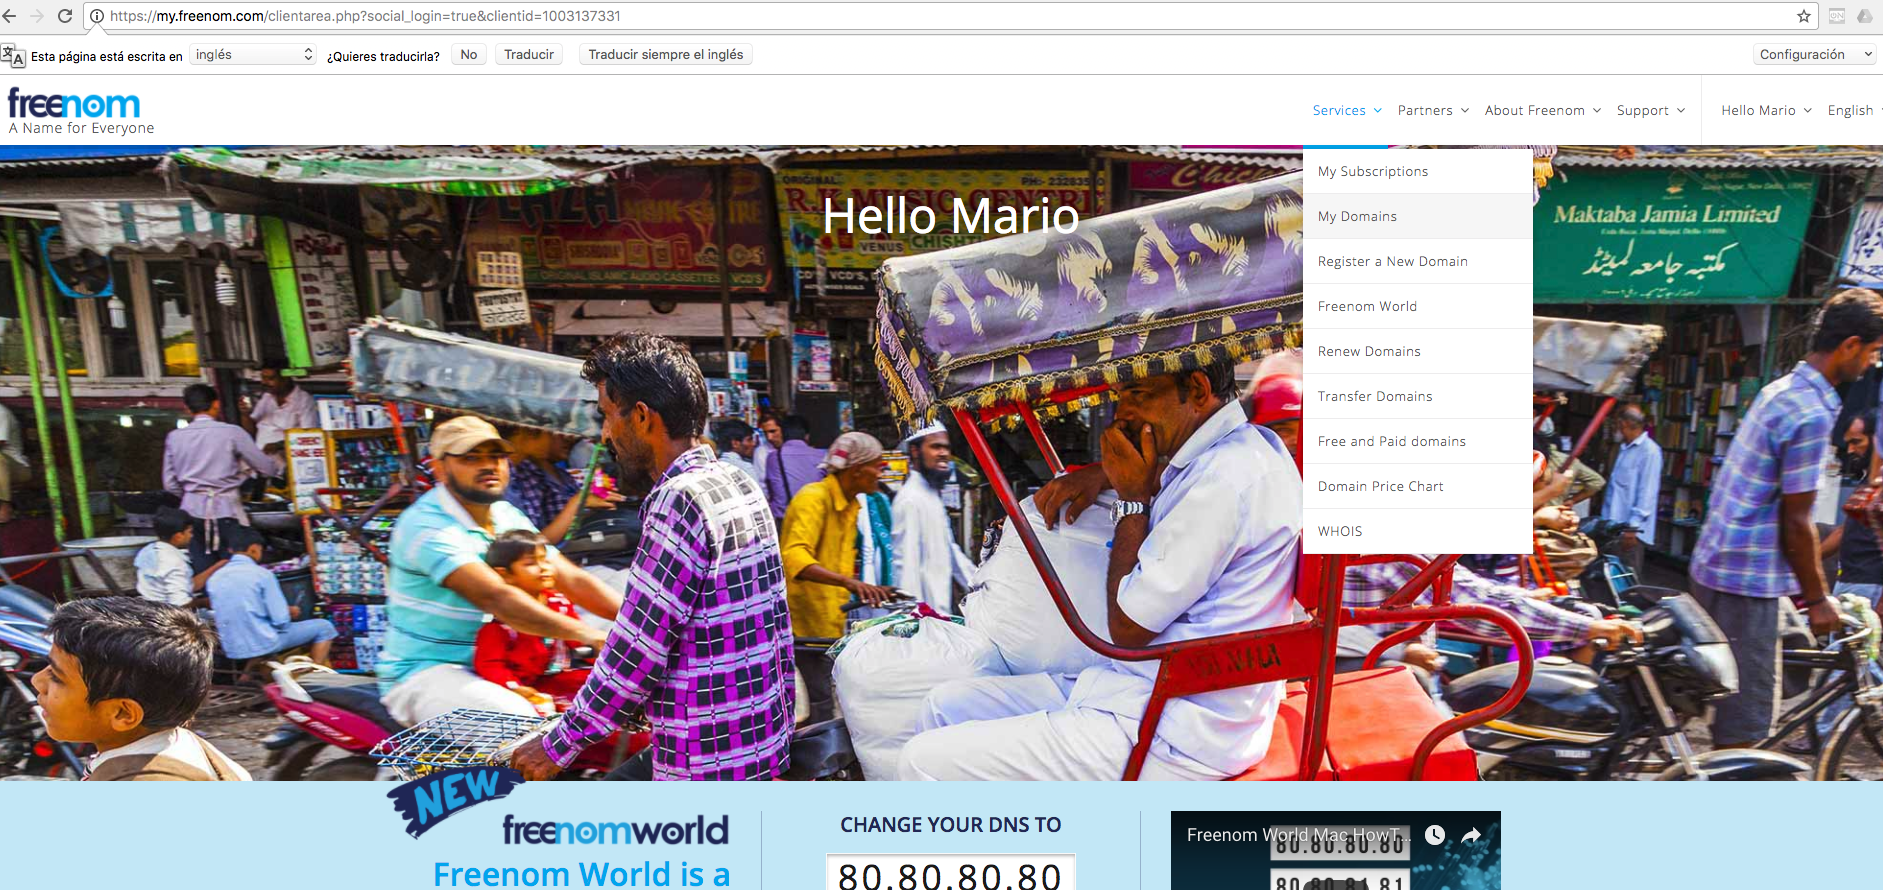
\includegraphics[width=80mm]{memoria/LaTeX/img/despliegue/dominiofree/paso1_2.png}
        \caption{Paso 1.2}
        \end{figure}
        \item En nuestro caso, el dominio elegido es www.classcity.tk. Una vez creado nuestro dominio, comenzamos la configuración haciendo click en el boton Manage Domain.
        \begin{figure}[H]
        \centering
        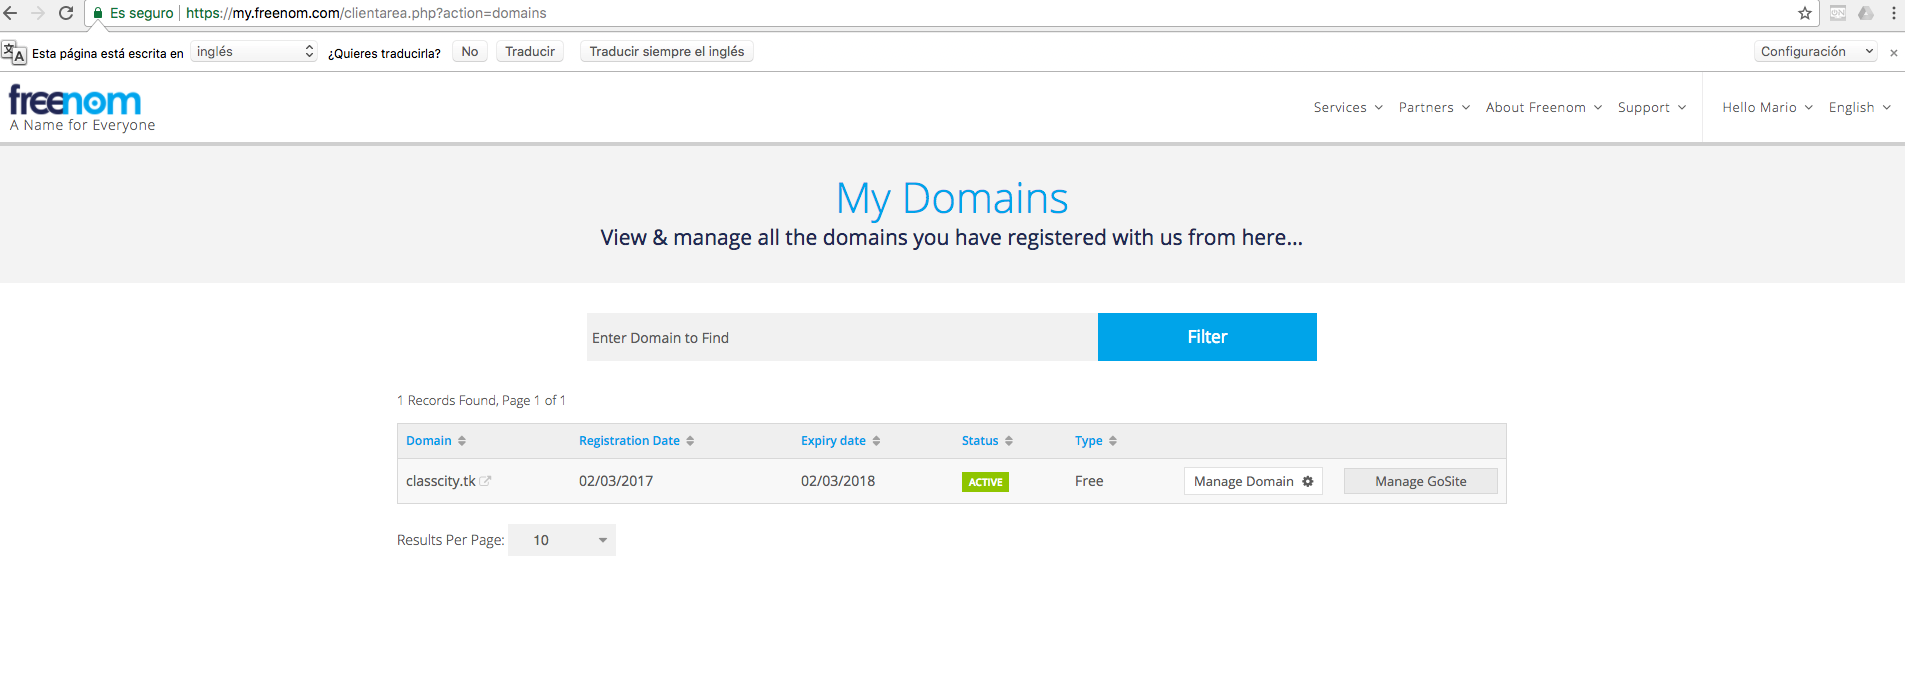
\includegraphics[width=80mm]{memoria/LaTeX/img/despliegue/dominiofree/paso1_3.png}
        \caption{Paso 1.3}
        \end{figure}
        \item Dentro del Managin del dominio, nos vamos a la seccion Manging Tools, y hacemos click en nameerver tal y como se puede ver en la siguiente imagen,
        \begin{figure}[H]
        \centering
        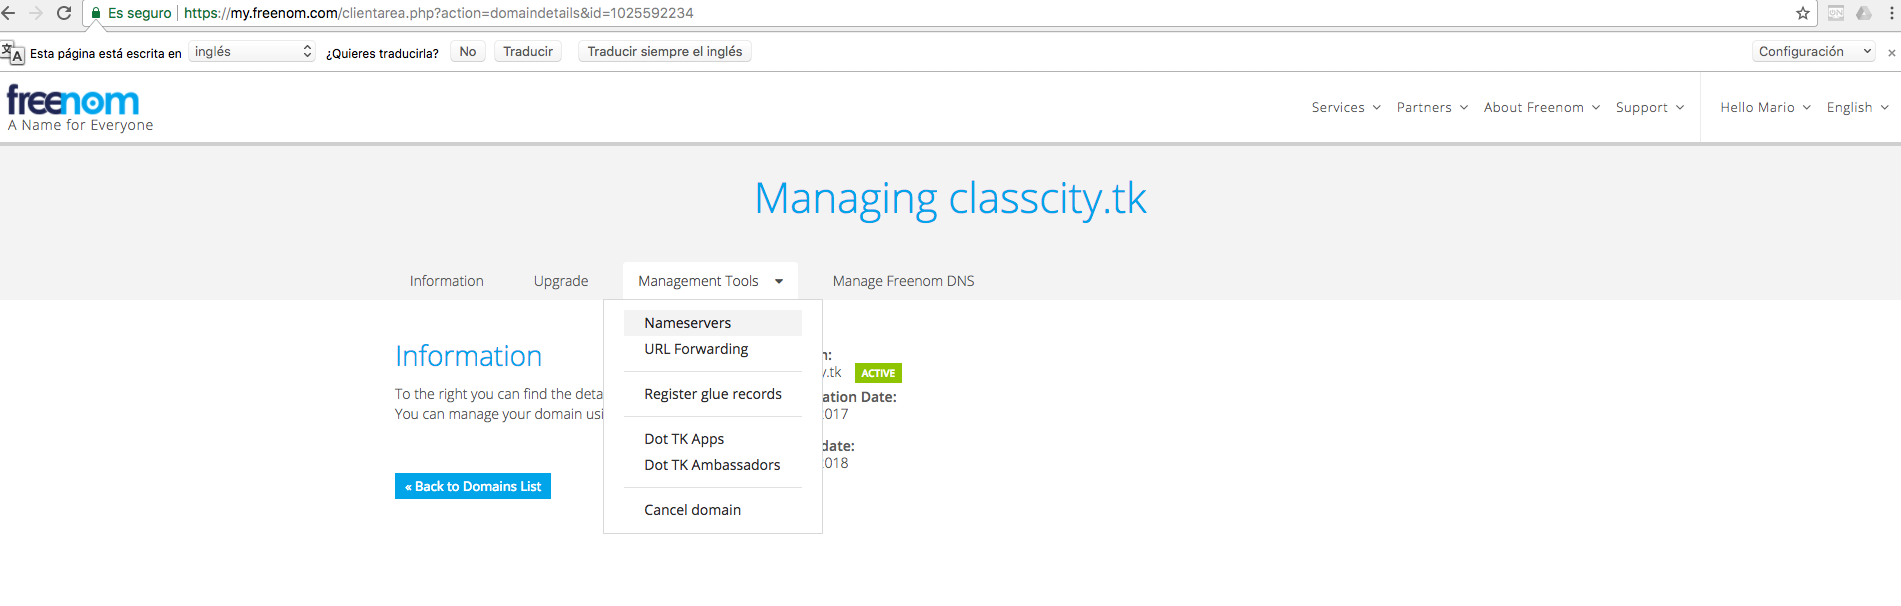
\includegraphics[width=80mm]{memoria/LaTeX/img/despliegue/dominiofree/paso1_4.png}
        \caption{Paso 1.4}
        \end{figure}
        \item Debe cambiar los servidores de nombres y seleccionar usar servidores de nombres personalizados.
        \begin{figure}[H]
        \centering
        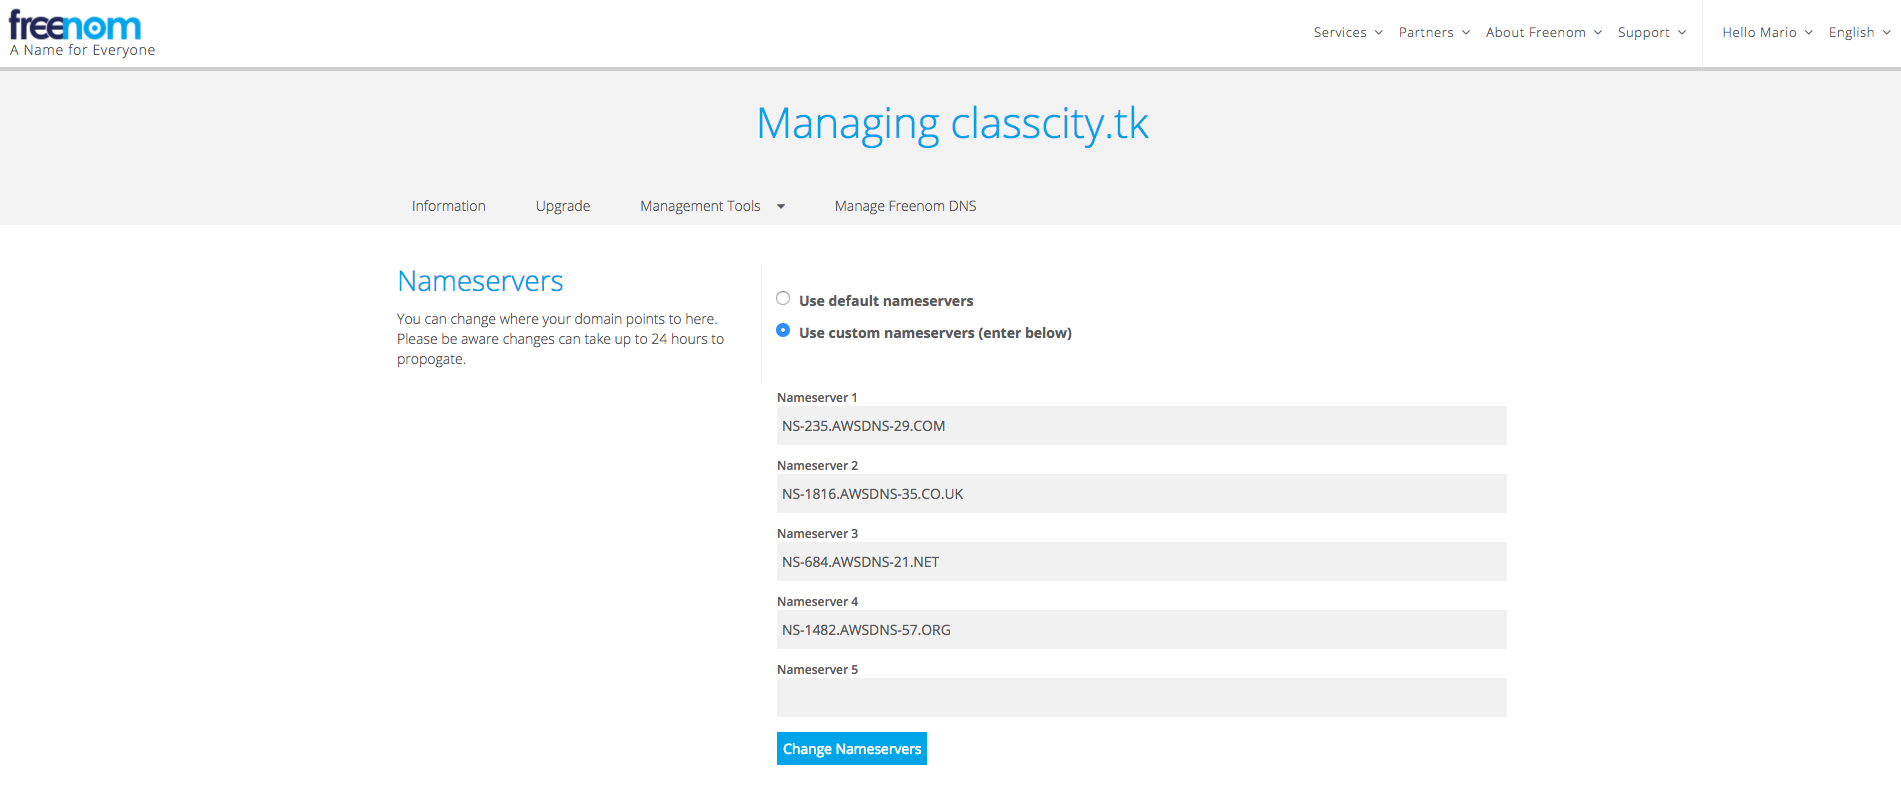
\includegraphics[width=80mm]{memoria/LaTeX/img/despliegue/dominiofree/paso1_5.png}
        \caption{Paso 1.5}
        \end{figure}
    \end{enumerate}
    
    \item \textbf{Paso 4. Obtener un certificado SSL gratis con AWS Certificate Manager para CloudFront} 
    
    Un certificado SSL es un fichero informático generado por una entidad de servicios de certificación que asocia unos datos de identidad a una persona física, organismo o empresa, confirmando de esta manera su identidad digital en Internet. Necesitamos un certificado SSL para que los usuarios que accedan a nuestra página lo hagan de una forma segura por el protocolo HTTPS.
    
    Por otro lado tenemos Amazon CloudFront, es un servicio de red de entrega de contenido (CDN) global que proporciona datos, vídeos, aplicaciones y API de forma segura a sus espectadores con baja latencia y altas velocidades de transferencia. 
    
    Para conseguir el certificado SSL en AWS necesitas seguir los siguientes pasos:
    
    
     \begin{enumerate}
        \item Tienes que ir a AWS manager certificate desde la consola de Amazon web services y hacer click en get started.
        \item A continuación te pedirá el dominio creado previamente y tendrás que hacer click en Review and request.
        \item Una vez enviado la solicitud de certificado a la Autoridad certificadora, un email de confirmación será enviada a nuestra cuenta de correo vinculada con el dominio, es decir a admin@classcity.tk. En nuestro caso como disponemos de un dominio gratuito debemos hacer una redirección desde el portal http://www.tkmailias.tk/es/pageA00E1.html, y desde allí conseguir redireccionar nuestra cuenta admin@classcity.tk a un correo personal, para recibir la confirmación del certificado.
        \item Una vez que recibimos un correo como el que aparece en la siguiente imagen, realizamos la confirmación del certificado haciendo click en el enlace que viene en el correo
        \begin{figure}[H]
        \centering
        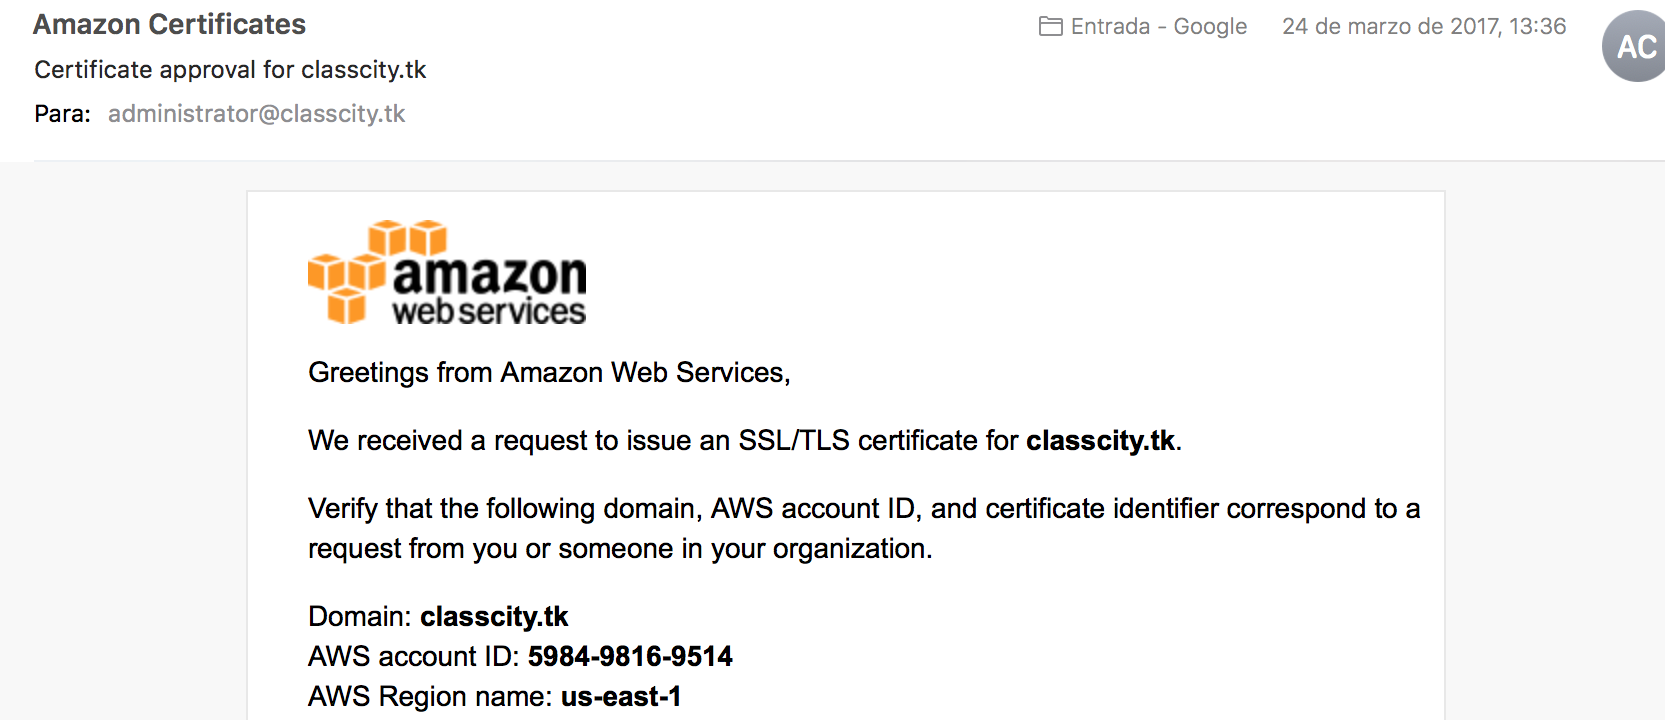
\includegraphics[width=80mm]{memoria/LaTeX/img/despliegue/ssl.png}
        \caption{Correo de confirmación}
        \end{figure}
    \end{enumerate}
    
    Una vez que tenemos el certificado SSL generado es momento de configurar cloudfront proporcionándole de dicho certificado, para ello debemos seguir los siguientes pasos:
    
    \begin{enumerate}
    \item Buscar cloudfront desde la consola de AWS. 
    \item Una vez alli debemos crear una distribucion
    \item En el momento de elegir la configuracion del SSL certificate, marcaremos la opcion Custom SSL Certificate, tal y como podemos ver en la siguiente imagen.
    \begin{figure}[H]
    \centering
    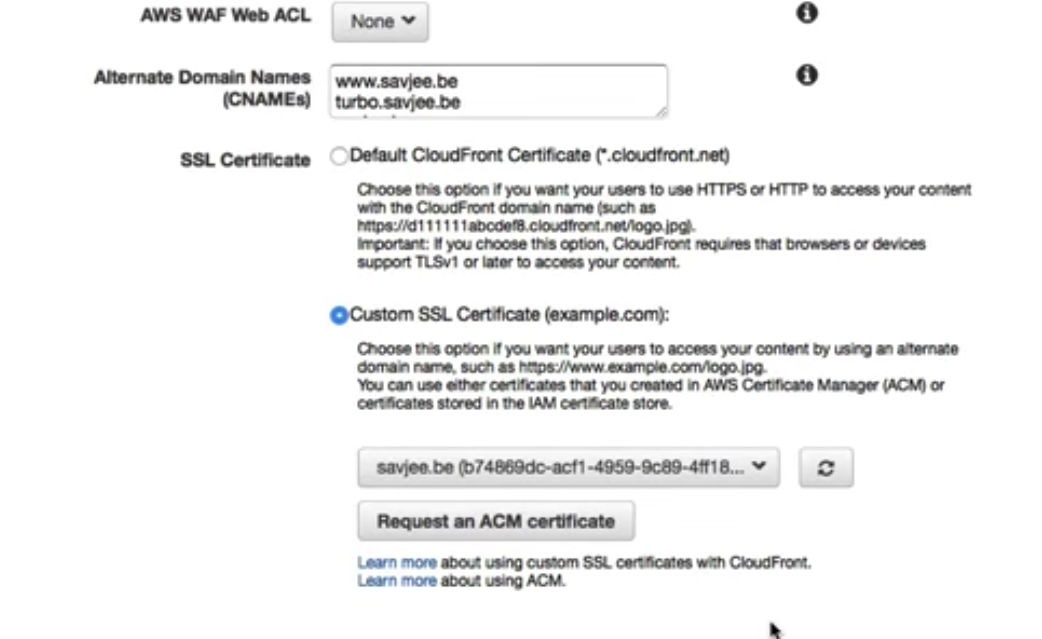
\includegraphics[width=80mm]{memoria/LaTeX/img/despliegue/customssl.png}
    \caption{SSL}
    \end{figure}
    \end{enumerate}
    
    Si ahora vamos a nuestro dominio e introducimos antes el protocolo HTTPS, es decir en nuestro caso https://www.classcity.tk, veremos que efectivamente accedemos a nuestra aplicacion de una forma segura.  

    \begin{figure}[H]
    \centering
    
\includegraphics[width=80mm]{memoria/LaTeX/img/despliegue/https.png}
    \caption{SSL}
    \end{figure}

\end{itemize}
    
\section{Lanzar una aplicación MEAN a producción} Una vez que dispongamos de una instancia, un dominio, un certificado SSL y una distribución cloufront, tenemos todo listo para poder desplegar nuestra aplicación MEAN en producción. Para ello debemos seguir los siguientes pasos:

\begin{enumerate}
    \item Conectarnos desde nuestra terminal por SSH a nuestra maquina virtual de AWS
    \begin{lstlisting}
    sudo ssh -i /.ssh/keypair.pem root@ipinstance
    \end{lstlisting}
    \item Clonar en la maquina virtual de AWS, nuestro repositorio git donde almacenemos la aplicación MEAN.
    \begin{lstlisting}
    rooti@ip sudo git clone https//github.com/RoboticsURJC-students/2016-tfg-Mario-Fernandez.git 
    \end{lstlisting}
    \item Instalar dependecias de la aplicacion web por parte del Front-End
    \begin{lstlisting}
    rooti@ip cd 2016-tfg-Mario-Fernandez
    rooti@ip /2016-tfg-Mario-Fernandez sudo npm install
    \end{lstlisting}
    \item Correr Angular2 con angular-ci
    \begin{lstlisting}
    rooti@ip /2016-tfg-Mario-Fernandez sudo npm run build
    \end{lstlisting}
    \item Una nueva carpeta se crea al terminar el proceso ./dist, debemos copiarla entera en nuestra carpeta httdocs de apache.
    \begin{lstlisting}
    rooti@ip /2016-tfg-Mario-Fernandez sudo cp -r ./dist/* ../httdocs
    \end{lstlisting}
    \item Ahora deberíamos poder ir a https://www.classcicty.tk y poder ver nuestra aplicación Angular2 corriendo en producción.
     \begin{figure}[H]
    \centering
    
\includegraphics[width=80mm]{memoria/LaTeX/img/templates/intro.png}
    \caption{https://www.classcity.tk}
    \end{figure}
    \item No olvidemos que en el stack MEAN, aun falta que configuremos el servidor en producción. Para ello lo primero es instalar las dependencias necesarias para el backend.
    \begin{lstlisting}
    rooti@ip /2016-tfg-Mario-Fernandez cd backend
    rooti@ip /2016-tfg-Mario-Fernandez/backend sudo npm install
    \end{lstlisting}
    \item Antes de ponernos a ejecutar nada en la parte del backend, debemos configurar ciertas rutas en nuestro servidor apache que va ser el encargado de recibir la peticiones de entrada. Para ello debemos hacer lo siguiente:
    \begin{itemize}
    
        \item  Editamos el archivo de configuración de apache llamado httpd.conf para que cuando llegue las solicitudes de tipo / app / * redirigir a localhost: 8080, que será donde estará escuchando nuestra aplicación.
        \begin{lstlisting}
        ProxyPassMatch ^/app/(.*)$ http//localhost:8080/$1
        ProxyPass /app/(.*)$ http//localhost:8080/
        ProxyPassReverse /app/(.*)$ http//localhost:8080/
        \end{lstlisting}
        \item Y cuando llega la solicitud de type / socket / * redirigir a localhost: 8000, que será el puerto donde este escuchando nuestro chat.
        \begin{lstlisting}
        ProxyPassMatch ^/socket/(.*)$ http//localhost:8000/$1
        ProxyPass /socket/(.*)$ http//localhost:8000/
        ProxyPassReverse /socket/(.*)$ http//localhost:8000/
        \end{lstlisting}
    \end{itemize}
   
    \item A continuación en el backend correremos la base de datos con la propiedad screen, para que cuando se termine la conexión por ssh el proceso siga corriendo y no se corte.
    \begin{lstlisting}
    rooti@ip /2016-tfg-Mario-Fernandez/backend sudo mkdir data
    rooti@ip /2016-tfg-Mario-Fernandez/backend sudo screen mongod --dbpath ./data
    \end{lstlisting} 
    \item Y por último ejecutamos e fichero server.js también con la propiedad screen, y comprobaremos que funciona correctamente.
    \begin{lstlisting}
     rooti@ip /2016-tfg-Mario-Fernandez/backend sudo node server.js screen
    \end{lstlisting} 
\end{enumerate}